\chapter{The mesh}

\devnote{This chapter is currently being written\ldots}

% FIXME: Triangular, tetrahedral, include some images,
% FIXME: mesh refinement, connectivity, iterators, file formats, local
% FIXME: ordering

The concept of a \emph{mesh} is central in the implementation of
adaptive Galerkin finite element methods for partial differential equations.
Other important concepts include \emph{nodes}, \emph{cells},
\emph{edges}, \emph{faces}, \emph{boundaries}, and \emph{mesh hierarchies}. These 
concepts are all implemented as C++ classes in \dolfin{}, as shown in Figure \ref{fig:meshclasses}.

\begin{figure}[htbp]
  \begin{center}
    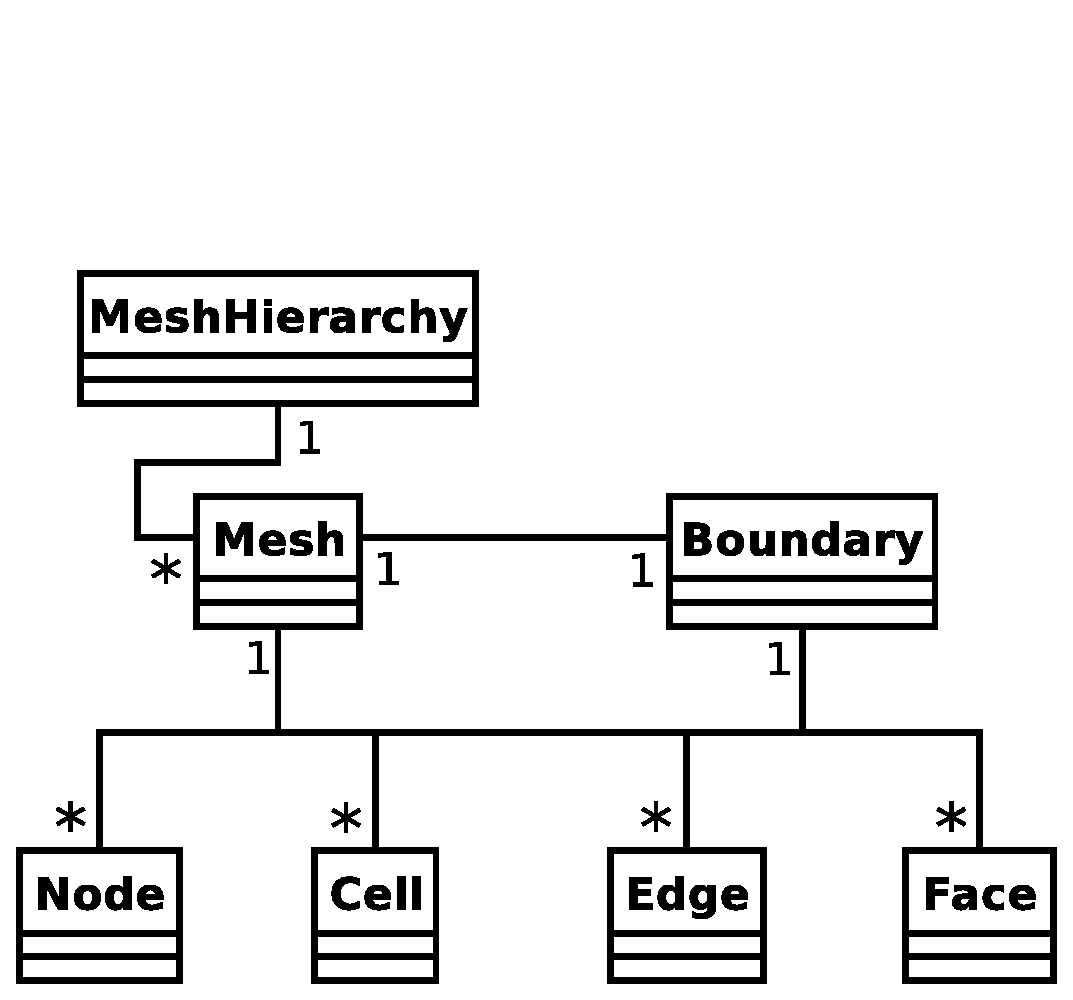
\includegraphics[width=10cm]{eps/mesh-components.eps}
    \caption{Class diagram of the basic mesh classes in \dolfin{}.}
    \label{fig:meshclasses}
  \end{center}
\end{figure}

Algorithms operating on a mesh, including adaptive mesh refinement,
can often be expressed in terms of
\emph{iterators}, i.e., objects used for the traversal of aggregate
structures, such as the list of nodes contained in a mesh. Iterators
implemented in \dolfin{} include a \texttt{NodeIterator},
\texttt{CellIterator}, \texttt{Edge}\-\texttt{Iterator}, \texttt{FaceIterator},
and a \texttt{MeshIterator}. Table \ref{tab:iterators} provides an example of a code that
displays all node neighbors of all nodes of all cells within a
given mesh.

\begin{table}[htbp]
\begin{code}
  for (CellIterator c(m); !c.end(); ++c)
    for (NodeIterator n1(c); !n1.end(); ++n1)
      for (NodeIterator n2(n1); !n2.end(); ++n2)
        cout << *n2 << endl;
\end{code}
\caption{Iteration over all node neighbors \texttt{n2} of the nodes
\texttt{n1} within all cells \texttt{c} of the mesh \texttt{m}.}
\label{tab:iterators}
\end{table}

Adaptive mesh refinement is implemented in \dolfin{} for triangular
meshes (in 2D) and tetrahedral meshes (in 3D), see Figure
\ref{fig:refinedmeshes}, based on the algorithm given in \cite{Bey95}.
To refine a mesh, the cells (triangles or tetrahedrons) are first
marked according to some criterion for refinement, before the mesh is
refined. A hierarchy of meshes, that can be used for example in a
multigrid computation, is automatically created.

\begin{figure}
  \begin{center}
    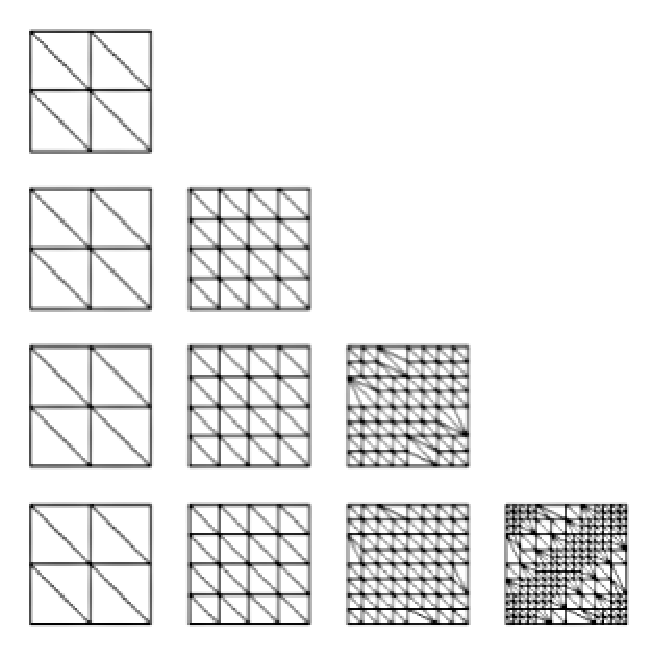
\includegraphics[width=6cm]{eps/mesh2d.eps}
    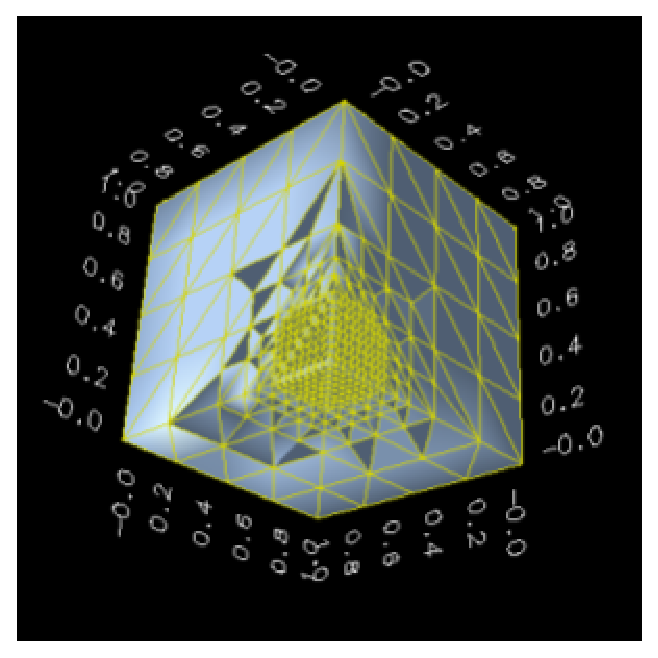
\includegraphics[width=6cm]{eps/mesh3d.eps}
    \caption{Adaptive mesh refinement of triangular and tetrahedral meshes in \dolfin{}.}
    \label{fig:refinedmeshes} 
  \end{center}
\end{figure}

\begin{table}
\begin{code}
  // Mark cells for refinement
  for (CellIterator cell(mesh); !cell.end(); ++cell)
    if ( ... )
      cell->mark();

  // Refine mesh
  mesh.refine();
\end{code}
\caption{Sketch of adaptive mesh refinement in \dolfin{}.}
\label{tab:refinement}
\end{table}
